\subsection{Introduction}
\label{subsec:introduction3}

Over the years, GPUs have served as the primary hardware accelerators for deep learning workloads,
offering significant performance improvements over traditional CPUs.
This has been further aided by the development of specialized software for high-performance deep learning such as cuDNN and cuBLAS for NVIDIA GPUs and ROCm for AMD GPUs.
Only recently, however, TPUs (and TensorFlow) have emerged as a viable alternative to GPUs for deep learning tasks.
However,
different generations of AI accelerators across different vendors exhibit vastly different performance and energy consumption characteristics.
Even with similar on-paper specifications like core clocks, Video random-access memory (VRAM), memory bandwidth,
the real-life performance relies heavily on an accelerator's underlying architecture and
software (driver) optimizations.

Additionally, for server-based deployment,
monitoring energy consumption has been vital for DNN training,
since long-term electric bills can directly benefit from lower energy consumption.
There exist techniques to balance performance and energy consumption such as dynamic voltage and frequency
(DVFS)\cite{b1} and job scheduling algorithms like First Come, First Served (FCFS) or Shortest Job First (SJF)\cite{b2}, etc.

Most existing benchmarks exclusively consider either performance or energy consumption for particular accelerators and/or algorithms.
Also, there is limited data available for AMD GPUs, despite significant improvements to the ROCm ecosystem.
Hence, for the purposes of this work,
wide benchmarks for CIOs and real-world tasks such as image recognition,
speech recognition and translation tasks are made.

\subsection{Preliminaries}
\label{subsec:prelims}
\subsubsection{Deep Models}
There exist various types of state-of-the-art deep architectures.
Convolutional Neural Networks (CNNs) are preferred for image classification and object detection tasks,
among which VGG, ResNet, and Inception are widely used.

\begin{figure}[htbp!]
    \centering
    {    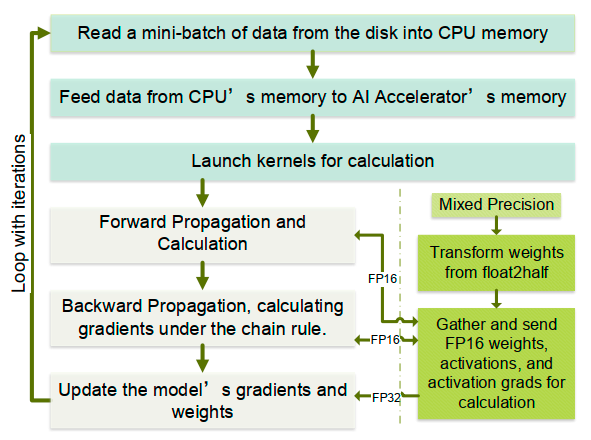
\includegraphics[width=0.5\textwidth]{images/training_pipeline}}
    \caption{The training pipeline of deep neural networks. Note that FP16 will be replaced by bfloat16 when training DNNs on TPUs.}
    \label{fig:pipeline}
\end{figure}

\subsubsection{Mixed Precision Training}
The mixed precision training technique uses low-bit floating points to forward and backward during training
to maximize hardware utilization.
Typically, in mixed precision, FP32 master weights and loss scaling are adopted to avoid FP16's instability.
``Fig. \ref{fig:pipeline}'' shows the training pipeline for DNNs.

\begin{table*}[h!]
    \centering
    \setlength\tabcolsep{8pt}
    \caption{Hardware Setup}
    \label{tab:hardware}
    \begin{tabular}{c c c c c c c}
        \toprule
        Vendor & Accelerator Model & Memory & Theoretical FLOPS   & Memory Bdw & Memory Type & CPU      \\
        \midrule
        NVIDIA & Titan X(Pascal)   & 12 GB  & 11 T (FP32)         & 480.4 GB/s & GDDR5X      & i7-7820X \\
        & Tesla P100        & 16 GB  & 9.5 T (FP32)        & 732.2 GB/s & HBM2        & i7-6800K \\
        & Tesla V100        & 16 GB  & 112 T (Tensor Core) & 897.0 GB/s & HBM2        & i7-6800K \\
        AMD    & Radeon VII        & 16 GB  & 13.44 T (FP32)      & 1 TB/s     & HBM2        & i7-4790  \\
        Google & TPU v2-8          & 64 GB  & 180 T (bfloat16)    & 600 GB/s   & HBM         & -        \\
        & TPU v3-8          & 128 GB & 420 T (bfloat16)    & 900 GB/s   & HBM         & -        \\
        \bottomrule
    \end{tabular}
\end{table*}

\subsubsection{Hardware Setup}
Many-core processors from NVIDIA, AMD, and Google are selected for evaluation.
For each vendor, one to three processors are included.
The details are presented in ``Table~\ref{tab:hardware}''.

\subsection{Experimental Results}
\label{subsec:results}
\subsubsection{Performance of Computation-intensive operations}

\begin{figure}[htbp!]
    \centering
    {    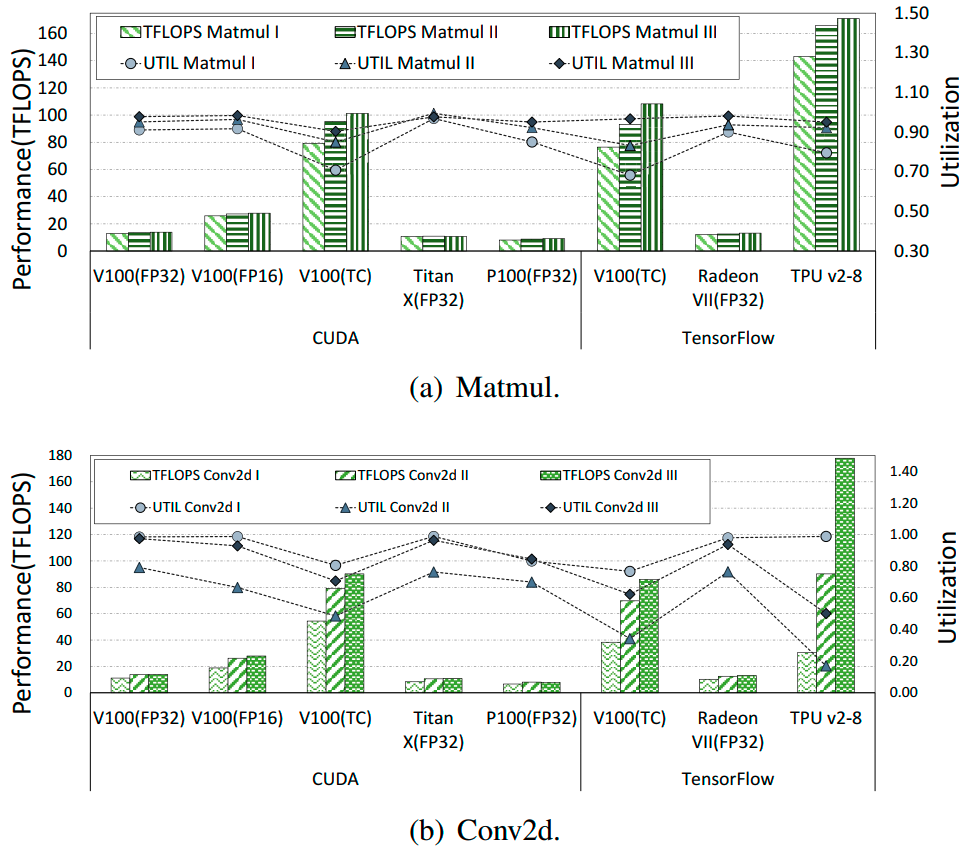
\includegraphics[width=0.5\textwidth]{images/cios_gpu_tpu}}
    \caption{The results of GPU and TPU’s performance (FLOPS) and utilization of Matmul and Conv2d operators.}
    \label{fig:cios}
\end{figure}

\begin{table*}[t]
    \centering
    \setlength\tabcolsep{8pt}
    \caption{The Average Utilization of TensorCore}
    \begin{tabular}{c c c c c c c}
        \toprule
        DNNs             & Resnet50 & Inception v3 & Vgg16 & 2-LayerLSTM & DeepSpeech2 & Transformer \\
        \midrule
        Tensor Core Util & 9.2\%    & 6.8\%        & 7.3\% & 3.9\%       & 5.1\%       & 4.4\%       \\
        \bottomrule
    \end{tabular}
    \label{tab:tensorutil}
\end{table*}

The GPU and TPU performance and utilization results are shown in ``Fig. \ref{fig:cios}''.
Among GPUs, P100 has the lowest utilization under all observed workloads.
V100 achieves a high 97\% utilization for Matmul and 92\% for Conv2d under FP32/FP16 precision.
With Tensor cores enabled, the utilization of V100(TC) is lower than V100(FP32) by approximately 20\%.
High-throughput kernels are used in computation-intensive operations to maximize FLOPS (throughput), as illustrated in ``Fig. \ref{fig:cios}''.
The performance gap between the CUDA C++ and TensorFlow implementations on Tensor Core is more significant for Conv2d than Matmul.
Among GPUs, V100, Titan X, and Radeon VII all achieve optimal FP32 performance and utilization on both operators, demonstrating their high-throughput computing capabilities.
TPU V2 nearly reaches full utilization on both operators, with an impressive 99\% on the Conv2d operator, which is significantly better than Tesla V100 with Tensor Core.
Therefore, it can be concluded that performance bottlenecks still exist for V100 when Tensor Core is enabled.

\subsubsection{Performance of End-to-end Training}

\begin{figure}[htbp!]
    \centering
    {    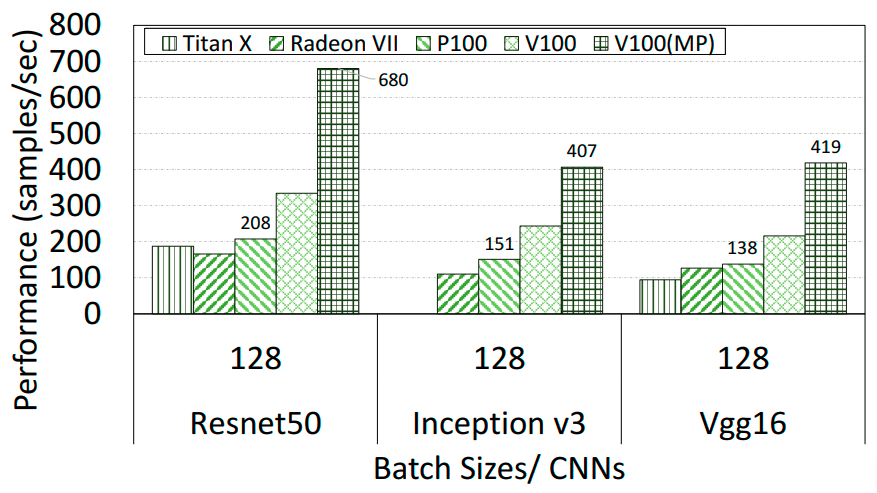
\includegraphics[width=0.5\textwidth]{images/gpucnn}}
    \caption{The results of performance comparison on GPUs with CNNs. Note that the Titan X GPU runs out of memory when training inception v3 and batchsize = 128.}
    \label{fig:cnn}
\end{figure}

As depicted in ``Fig. \ref{fig:cnn}'', among the GPUs tested, Tesla V100 delivers the highest performance for both FP32 and Mixed Precision training.
When compared under the same numerical precision, NVIDIA V100 typically outperforms the AMD Radeon VII GPU by a factor of 1.5 to 2.
Tesla P100 and Titan X (Pascal), both from NVIDIA, demonstrate similar performance levels, which can be attributed to their comparable peak FLOPS and memory bandwidth, as detailed in ``Table \ref{tab:hardware}''.
However,
the advantage of switching from FP32 Precision to Mixed Precision results in a maximum of 2x higher throughput for V100,
with Tensor Core utilization reaching only 9\% at most on Resnet50,
as per ``Table \ref{tab:tensorutil}'' - a figure significantly lower than the peak FLOPS.
Comparing the two desktop-level GPUs, NVIDIA Titan X (Pascal) and AMD Radeon VII,
the latter's peak FLOPS and memory bandwidth are approximately 22\% and 52\% higher than the former's, respectively.
Despite this, Titan X slightly outperforms Radeon VII on Resnet 50.
This suggests that there is room for further optimization in the AMD software ecosystem to better leverage the hardware capabilities for various deep learning workloads.

\subsection{Evaluation}
\label{subsec:evaluation}
\subsubsection{Comparison between GPU and TPU}

\begin{figure}[htbp!]
    \centering
    {    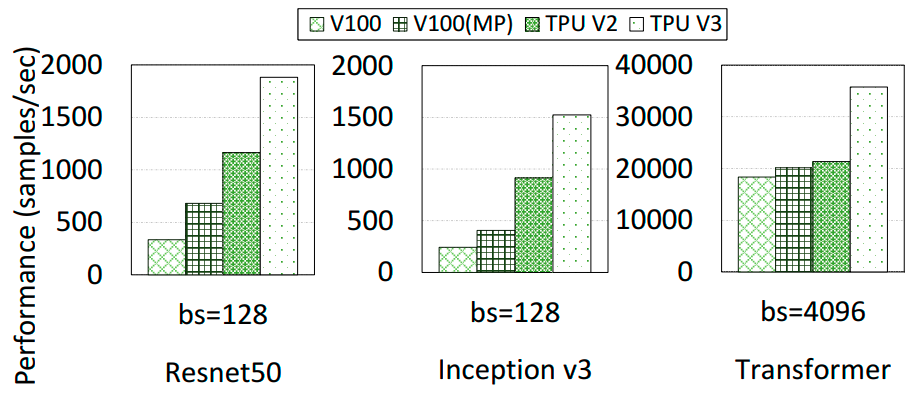
\includegraphics[width=0.5\textwidth]{images/tpugpucomp}}
    \caption{The results of performance comparison between Tesla V100 GPU and TPUs.}
    \label{fig:tpugpucomp}
\end{figure}

TPUs and Tesla V100 are among the world's fastest AI accelerators.
As shown in ``Fig. \ref{fig:tpugpucomp}'', TPUs surpass the Tesla V100 GPU in performance for the three models evaluated.
TPU V2 and TPU V3 offer 1.6x and 3.75x more FLOPS, but only 0.66x and equal memory bandwidth compared to V100, respectively.
When it comes to CNNs (ResNet-50 and Inception v3), TPU V2-8 and TPU V3-8 deliver over 1.5x and 2.7x higher throughput than Tesla V100 with Tensor Cores, respectively.
However, for the Transformer architecture, TPU V2-8's performance is nearly on par with the Tesla V100 GPU, while TPU V3-8 is approximately 1.7x faster than the Tesla V100.

\subsubsection{Limitation of Tensor Cores}
The Volta architecture optimizes the convolutional components in a neural network into matrix computations, which are then processed by Tensor Cores using FP16 precision parallel calculations.
In end-to-end Mixed Precision training, Tesla V100 (PCIe) performs over twice as well as it does in FP32 training, despite only utilizing 9\% of the peak FLOPS of Tensor Core.
However, intensive calculations in models like Resnet50 and Transformer make up over 40\% of the total calculations.
This discrepancy could be attributed to several potential factors: the remaining FP32 low-throughput calculations in Mixed Precision training, the inherently low utilization of Tensor Core, and the limited memory bandwidth.